\section{Tauri}
\label{sec:tauri}
Tauri was first released at \displaydate{dateTauriRelease}~\cite{tauriRelease} and downloaded approx. $58\,000$ times\footnote{According to \url{https://npm-stat.com/charts.html?package=tauri&from=2019-12-31&to=2022-08-12}}.
It resulted as discontent of Electron from the Tauri Developers especially in case of resource consumption and security due to uncontrollable dependencies.
They criticized the enormous resource consumption even of the simplest applications as well as the fact, that Electron does not have control over their dependencies.
If Chromium encounters a zero-day-exploit and releases a patch, Electron has to include this patch and also release a newer versions.
This leads to the fact, that users of an Electron-based application have to update their whole electron version to close this security issue.
This timespan, between first fix of chromium and the users update of the applications, is a high vulnerability for attackers.
In this regard, the developers also criticized the power of the privileges Electron applications have, allowing attackers to have access to the entire hard drive of the user for example~\cite{tauri}.
But like Electron Tauri experienced increased attention, which as in~\ref{sec:electron} can be expressed numerically based on GitHub Statistics~\cite{GithubTauri}: \\ \\
\begin{tabular} {| c | c | c | c | c |}
    \label{tab:tauri:statistics}
    Stars      & Forks     & Watching & Used by    & Contributors \\ \hline
    $48\,200$ & $1\,200$ & $403$ & $3\,200$ & $182$
\end{tabular} \\ \\
But unlike Electron, Tauri uses the self developed core, called Tauri, which is written in Rust in combination with WRY, which serves as the rendering library.


\subsection{Architecture}
\label{subsec:tauri:architecture}
The architecture of Tauri is very similar to Electrons multiprocess model.
Tauri also relies on a main process, called \textbf{core} process and multiple rendering processes, called \textbf{webview} for performance as well as security reasons.
\figref{fig:tauri:model} shows the basic architecture of Tauris multiprocess model whereas each \texttt{webview} process is managed by the \texttt{core} process.
by the
\begin{figure}[ht]
    \centering
    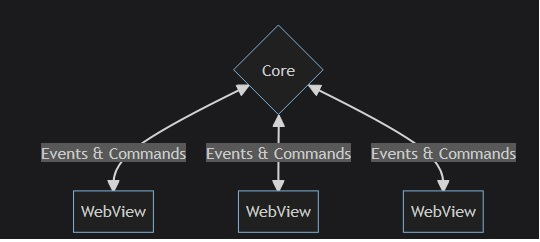
\includegraphics[width=0.4\textwidth]{images/TauriArchitecture}
    \caption{Multi-process Model Tauri from~\cite{tauri}}
    \label{fig:tauri:model}
\end{figure}

\begin{description}
    \item[\textbf{Core}:] \hfill \\ This is the main entry point of the application and the only place where full access to the operating system is provided.
    The \texttt{core} process uses this privileges to create and manage the windows the application.
    But it is also the only point, where the communication between processes is going through, allowing the core process to manipulate or observe \ac{IPC} messages.
    Additional the \texttt{core} process is responsible for global scoped cases such as database access or managing application or os-specific settings that affect the windows.
    Summarized it serves as a centralized management and control point, where the application as itself is maintained and sensitive data is kept to be hidden from the \texttt{webview} processes.


    \item[\textbf{WebView}:] \hfill \\ A \texttt{webview} process renders the ui by using the WebView libraries of the current os.
    Since this library is not included into the final executable but linked at runtime, it differs depending on the operating system the application is executed.
    This reduces the size of the executable since the part where the actual rendering takes places is shifted from the application to the operating system but also results
    that developers have to keep in mind the different operating systems.

\end{description}

\subsubsection{Inter Process Communication}
For communication between different processes Tauri also uses Inter Process Communication similar to Electron.
In contrast, Tauri forces developers from the beginning to use the \ac{AMP} paradigm, whereas Electron released this feature at version 14 and only recommends it.
The main advantage of \ac{AMP} is, that direct function access is denied and thus all communication has to go through the \texttt{core} process.
Since it is able to observe the content of messages, it can decide which message will be forwarded and which will be blocked like malicious requests.
Communication can be either unidirectional using events, which can be emitted by both \texttt{core} and \texttt{webview} processes to inform the event recipient but without any response,
or using commands which are bidirectional \ac{IPC} messages but can only be emitted by the \texttt{webview} processes to invoke functions that require access to the operating system.

\subsubsection{Context Isolation}
In contrast to Electron Tauri uses different patterns for isolating critical \ac{API} calls communication between the \texttt{webview} processes and the \texttt{core} process.
They are called Brownfield and Isolation Pattern, whereas the default pattern, that can be configured inside the \texttt{tauri.conf.json} is the Brownfield pattern
\begin{description}
    %TODO Brownfield pattern
    \item[\textbf{Brownfield Pattern}:] \hfill \\
    The Brownfield pattern can be seen as a design pattern to ensure interoperability between Tauri applications and existing frontend frameworks.
    Using the Brownfield pattern Tauri does not categorize existing frameworks as legacy software but instead as current state of the art and tries to adapt and fit to existing frameworks, whereas this is
    restricted by two types of
    \item[\textbf{Isolation Pattern}:] \hfill \\
    The Isolation Pattern can be seen as an interposed instance between the \ac{IPC} handler and the processes.
    This instance is providing a sandbox, called Isolation application, which is trusted and secure JavaScript code embedded into an \texttt{<iframe>}.
    The \ac{IPC} handler passes its message to the Isolation application, where it is executed and may be modified or verified.
    After that it will be encrypted, passed back to the \ac{IPC} handler and forwarded to the \texttt{core} process, where it will be handled as normal.


\end{description}
%Same as described for Tauri.Ref to introduction\ref{subsec:electron:arch}

\subsection{Frontend}
\label{subsec:tauri:frontend}
WRY and TAO
Webview implementierung
\subsection{Backend}
\label{subsec:tauri:backend}
TAURI CORE
ownership

